\begin{titlepage}
\thispagestyle{empty}
\normalfont
\begin{tikzpicture}[remember picture, overlay]
    % พื้นหลังหลักสีน้ำเงินเข้มและสีเขียวใบไม้ (Masterclass Geometry)
    \fill[rbruNavy] (current page.north west) rectangle (current page.south east);
    
    % แถบลายเส้นสีทองตัดระหว่างแถบหัว แถบกลาง และแถบล่าง
    \fill[rbruGold] ($(current page.north west)+(0,-5.4cm)$) rectangle ($(current page.north east)+(0,-5.7cm)$);
    \fill[agriGreen!80!black] ($(current page.north west)+(0,-5.7cm)$) rectangle ($(current page.south east)+(0,5.8cm)$);
    \fill[rbruGold] ($(current page.south west)+(0,5.8cm)$) rectangle ($(current page.south east)+(0,5.5cm)$);

    % วงกลมประดับออร่าเทคโนโลยีสีทองด้านหลังหน้าจอแดชบอร์ด (Grand Halo)
    \draw[rbruGold!35, line width=1.5pt] ($(current page.center)+(0,0.05cm)$) circle (7.4cm);
    \draw[rbruGold!20, line width=1pt, dashed] ($(current page.center)+(0,0.05cm)$) circle (8.0cm);

    % =========================================================================
    % 1. ชื่อหนังสือและตำราวิชาการด้านบนสุดของปก (Top Title Banner)
    % =========================================================================
    \node[anchor=north, text=white, align=center] at ($(current page.north)+(0,-1.15cm)$) {
        {\normalfont\fontsize{29}{35}\selectfont\bfseries JC -AGRITecH + AI Version 1.0}\\[7pt]
        {\normalfont\fontsize{18}{24}\selectfont\bfseries\color{rbruGold} คู่มือจัดทำระบบฟาร์มอัจฉริยะด้วยปัญญาประดิษฐ์และการเรียนรู้เชิงลึก}\\[5pt]
        {\normalfont\fontsize{13.5}{18}\selectfont\color{white} จากสมองกลฝังตัวสู่การพยากรณ์แปลงปลูกด้วย Deep Learning}
    };

    % =========================================================================
    % 2. ภาพประกอบหน้าจอแสดงผลหลัก Masterpiece UI ขยายขนาดใหญ่พิเศษ (18.0 cm x 12.0 cm)
    % =========================================================================
    \node[anchor=center] at ($(current page.center)+(0,0.05cm)$) {
        \begin{tikzpicture}
            % กรอบเงานุ่มลึก 3 มิติ (Soft Ambient Drop Shadow)
            \fill[black!60, rounded corners=14pt] (-8.95,-5.95) rectangle (9.05,5.85);
            % ภาพหน้าปัดตัดมุมโค้งมนขนาดใหญ่เต็มหน้ากระดาษ (18.0 cm x 12.0 cm)
            \begin{scope}
                \clip[rounded corners=12pt] (-9.0,-6.0) rectangle (9.0,6.0);
                \node at (0,0) {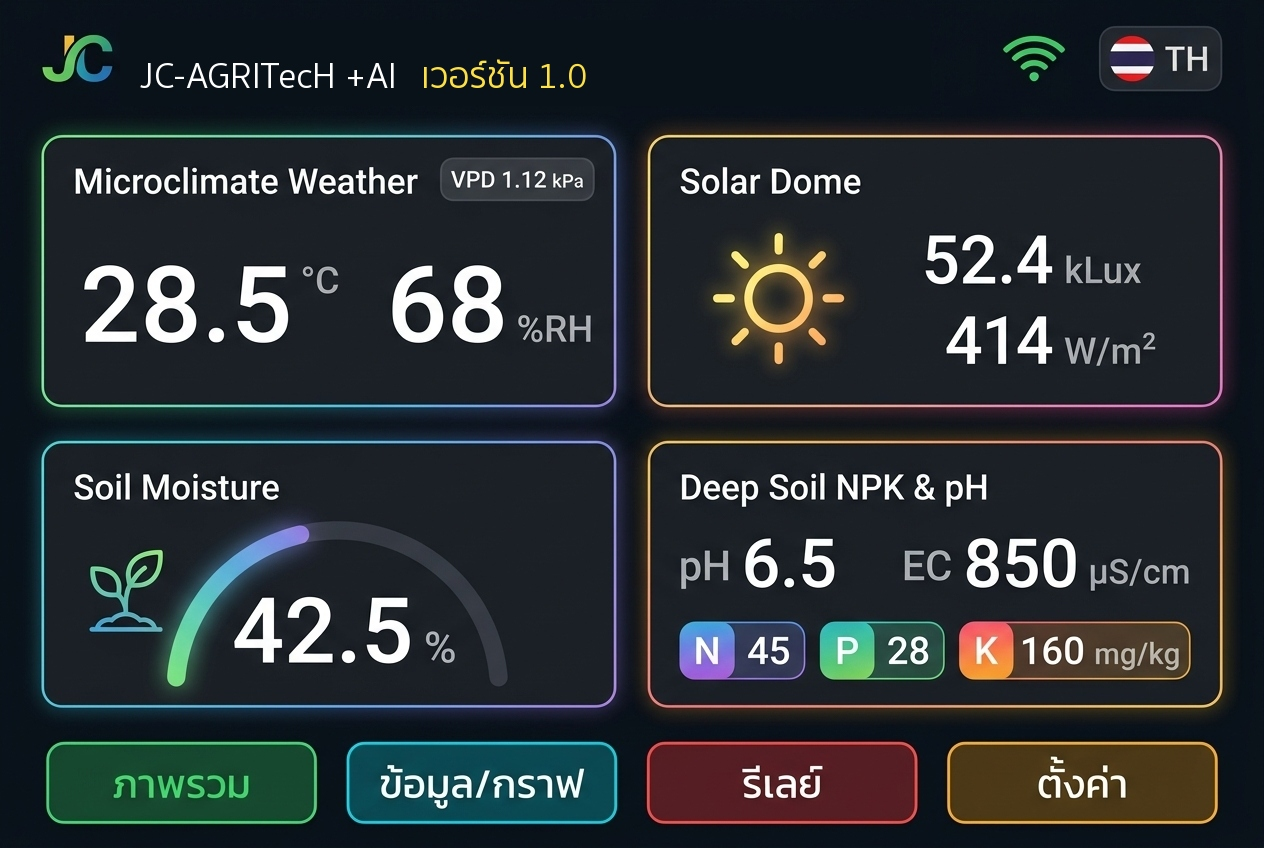
\includegraphics[width=18.0cm, height=12.0cm]{figures/smart_farm_ui_overview.jpg}};
            \end{scope}
            % ขอบสีทอง RBRU Gold หรูหรา ขนาด 3.5pt
            \draw[rbruGold, line width=3.5pt, rounded corners=12pt] (-9.0,-6.0) rectangle (9.0,6.0);
        \end{tikzpicture}
    };

    % =========================================================================
    % 3. ชื่อคณะผู้แต่งและตำแหน่งวิชาการ (Co-Authorship with Specific Disciplines)
    % =========================================================================
    \node[anchor=south, text=white, align=center] at ($(current page.south)+(0,2.0cm)$) {
        \begin{tabular}{c@{\hspace{1.2cm}}c}
            {\normalfont\fontsize{15}{19}\selectfont\bfseries ผู้ช่วยศาสตราจารย์ ดร.จิรภัทร จันทมาลี} & 
            {\normalfont\fontsize{15}{19}\selectfont\bfseries ผู้ช่วยศาสตราจารย์ ดร.ชีวะ ทัศนา}\\[3pt]
            {\normalfont\fontsize{13}{17}\selectfont\color{rbruGold} สาขาวิชาจุลชีววิทยา} & 
            {\normalfont\fontsize{13}{17}\selectfont\color{rbruGold} สาขาวิชาฟิสิกส์}\\[7pt]
            \multicolumn{2}{c}{{\normalfont\fontsize{13.5}{17.5}\selectfont คณะวิทยาศาสตร์และเทคโนโลยี มหาวิทยาลัยราชภัฏรำไพพรรณี}}
        \end{tabular}
    };

    % ปีที่พิมพ์
    \node[anchor=south, text=rbruGold] at ($(current page.south)+(0,0.85cm)$) {
        {\normalfont\fontsize{13.5}{17}\selectfont พ.ศ. 2569}
    };
\end{tikzpicture}
\end{titlepage}
\cleardoublepage
